% Created by tikzDevice version 0.8.1 on 2015-01-12 17:01:51
% !TEX encoding = UTF-8 Unicode
% Calculated string width of 0.0 as 12.263750
% Calculated character metrics. ascent: 6.611760, descent: 0.000000, width: 8.797910
% Calculated string width of 0.1 as 12.263750
% Calculated string width of 0.2 as 12.263750
% Calculated string width of 0.3 as 12.263750
% Calculated string width of military as 33.352080
% Calculated string width of monarchy as 40.816970
% Calculated string width of party as 22.421340
% Calculated string width of 0.00 as 17.062600
% Calculated string width of 0.25 as 17.062600
% Calculated string width of 0.50 as 17.062600
% Calculated string width of 0.75 as 17.062600
% Calculated string width of 1.00 as 17.062600
% Calculated string width of 0.00 as 17.062600
% Calculated string width of 0.25 as 17.062600
% Calculated string width of 0.50 as 17.062600
% Calculated string width of 0.75 as 17.062600
% Calculated string width of 1.00 as 17.062600
% Calculated string width of 0.00 as 17.062600
% Calculated string width of 0.25 as 17.062600
% Calculated string width of 0.50 as 17.062600
% Calculated string width of 0.75 as 17.062600
% Calculated string width of 1.00 as 17.062600
% Calculated string width of Proportion as 57.219210
% Calculated character metrics. ascent: 8.264620, descent: 0.000000, width: 10.997280
% Calculated string width of Estimated Probability as 116.404600
% Calculated string width of Proportion as 57.219210
% Calculated string width of Estimated Probability as 116.404600
% Drawing Rectangle from x0 = 0.000000, y0 = 0.000000 to x1 = 505.890000, y1 = 361.350000
% Beginning new tikzpicture 'page'
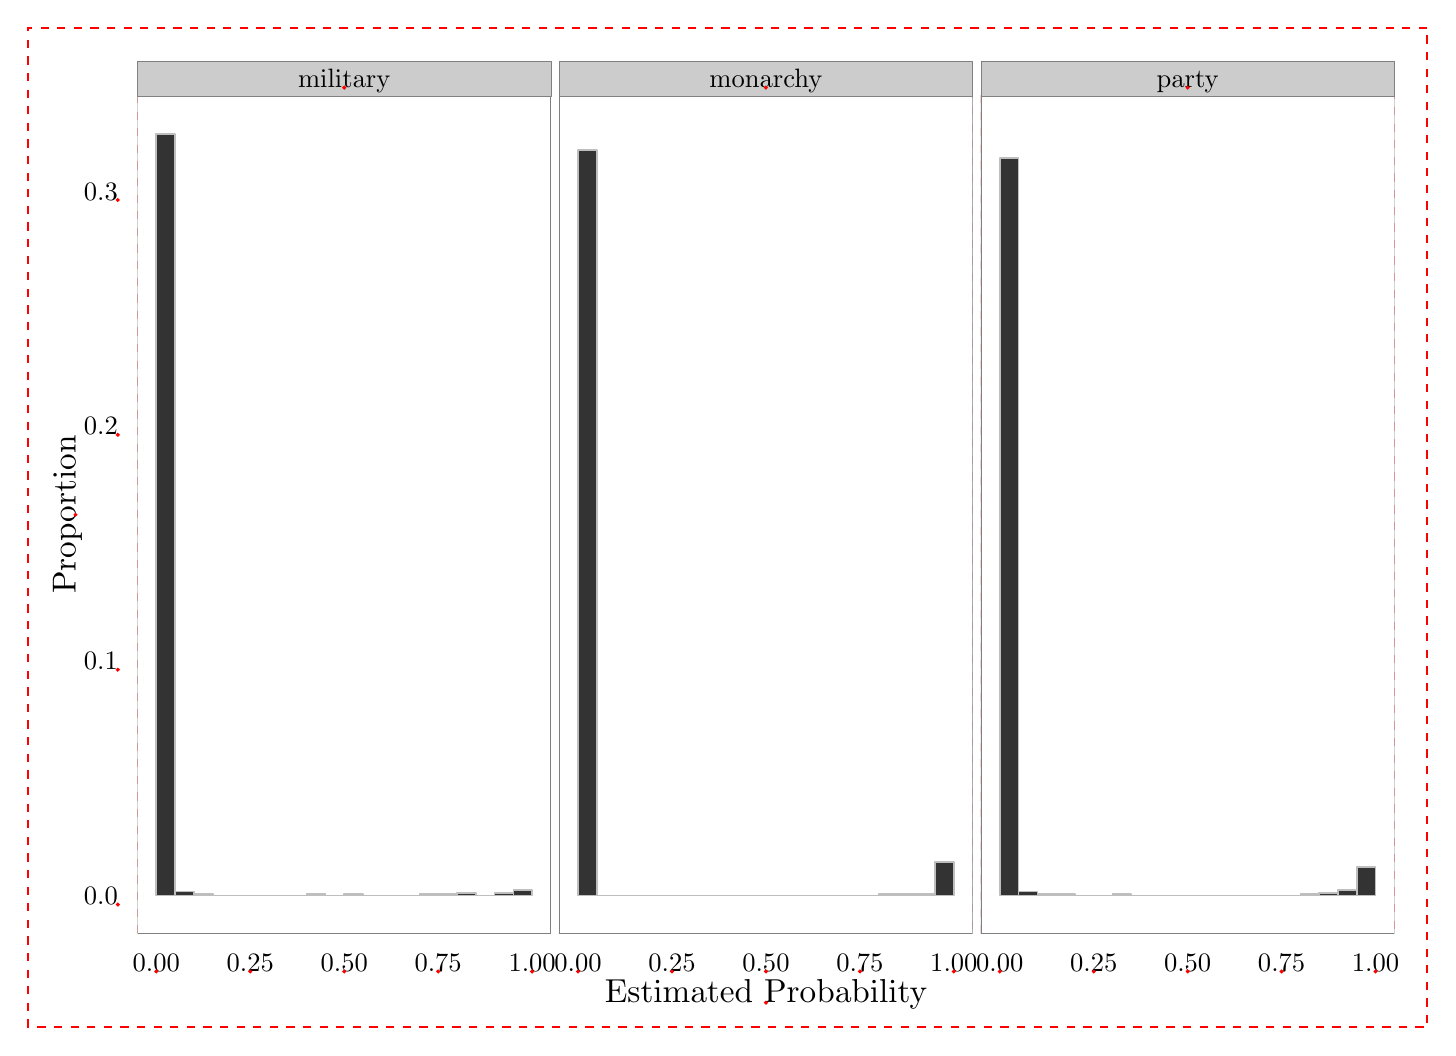
\begin{tikzpicture}[x=1pt,y=1pt]
\definecolor{fillColor}{RGB}{255,255,255}
\path[use as bounding box,fill=fillColor,fill opacity=0.00] (0,0) rectangle (505.89,361.35);
\begin{scope}
\path[clip] (  0.00,  0.00) rectangle (505.89,361.35);
\path[draw=red,very thick,dashed] (  0.00,  0.00) rectangle (505.89,361.35);
\definecolor{drawColor}{RGB}{255,255,255}
\definecolor{fillColor}{RGB}{255,255,255}

\path[draw=drawColor,line width= 0.6pt,line join=round,line cap=round,fill=fillColor] (  0.00,  0.00) rectangle (505.89,361.35);
\end{scope}
% Drawing Rectangle from x0 = 39.686559, y0 = 34.034569 to x1 = 189.065206, y1 = 336.670740
\begin{scope}
\path[clip] ( 39.69, 34.03) rectangle (189.07,336.67);
\path[draw=red,very thick,dashed] ( 39.69, 34.03) rectangle (189.07,336.67);
\definecolor{fillColor}{RGB}{255,255,255}

\path[fill=fillColor] ( 39.69, 34.03) rectangle (189.07,336.67);
% Drawing Rectangle from x0 = 46.476497, y0 = 47.790759 to x1 = 53.266436, y1 = 322.914550
\definecolor{drawColor}{RGB}{190,190,190}
\definecolor{fillColor}{gray}{0.20}

\path[draw=drawColor,line width= 0.6pt,line join=round,fill=fillColor] ( 46.48, 47.79) rectangle ( 53.27,322.91);
% Drawing Rectangle from x0 = 53.266436, y0 = 47.790759 to x1 = 60.056374, y1 = 49.246440

\path[draw=drawColor,line width= 0.6pt,line join=round,fill=fillColor] ( 53.27, 47.79) rectangle ( 60.06, 49.25);
% Drawing Rectangle from x0 = 60.056374, y0 = 47.790759 to x1 = 66.846313, y1 = 48.275986

\path[draw=drawColor,line width= 0.6pt,line join=round,fill=fillColor] ( 60.06, 47.79) rectangle ( 66.85, 48.28);
% Drawing Rectangle from x0 = 66.846313, y0 = 47.790759 to x1 = 73.636251, y1 = 47.790759

\path[draw=drawColor,line width= 0.6pt,line join=round,fill=fillColor] ( 66.85, 47.79) rectangle ( 73.64, 47.79);
% Drawing Rectangle from x0 = 73.636251, y0 = 47.790759 to x1 = 80.426190, y1 = 47.790759

\path[draw=drawColor,line width= 0.6pt,line join=round,fill=fillColor] ( 73.64, 47.79) rectangle ( 80.43, 47.79);
% Drawing Rectangle from x0 = 80.426190, y0 = 47.790759 to x1 = 87.216128, y1 = 47.790759

\path[draw=drawColor,line width= 0.6pt,line join=round,fill=fillColor] ( 80.43, 47.79) rectangle ( 87.22, 47.79);
% Drawing Rectangle from x0 = 87.216128, y0 = 47.790759 to x1 = 94.006067, y1 = 47.790759

\path[draw=drawColor,line width= 0.6pt,line join=round,fill=fillColor] ( 87.22, 47.79) rectangle ( 94.01, 47.79);
% Drawing Rectangle from x0 = 94.006067, y0 = 47.790759 to x1 = 100.796005, y1 = 47.790759

\path[draw=drawColor,line width= 0.6pt,line join=round,fill=fillColor] ( 94.01, 47.79) rectangle (100.80, 47.79);
% Drawing Rectangle from x0 = 100.796005, y0 = 47.790759 to x1 = 107.585944, y1 = 48.275986

\path[draw=drawColor,line width= 0.6pt,line join=round,fill=fillColor] (100.80, 47.79) rectangle (107.59, 48.28);
% Drawing Rectangle from x0 = 107.585944, y0 = 47.790759 to x1 = 114.375882, y1 = 47.790759

\path[draw=drawColor,line width= 0.6pt,line join=round,fill=fillColor] (107.59, 47.79) rectangle (114.38, 47.79);
% Drawing Rectangle from x0 = 114.375882, y0 = 47.790759 to x1 = 121.165821, y1 = 48.275986

\path[draw=drawColor,line width= 0.6pt,line join=round,fill=fillColor] (114.38, 47.79) rectangle (121.17, 48.28);
% Drawing Rectangle from x0 = 121.165821, y0 = 47.790759 to x1 = 127.955759, y1 = 47.790759

\path[draw=drawColor,line width= 0.6pt,line join=round,fill=fillColor] (121.17, 47.79) rectangle (127.96, 47.79);
% Drawing Rectangle from x0 = 127.955759, y0 = 47.790759 to x1 = 134.745698, y1 = 47.790759

\path[draw=drawColor,line width= 0.6pt,line join=round,fill=fillColor] (127.96, 47.79) rectangle (134.75, 47.79);
% Drawing Rectangle from x0 = 134.745698, y0 = 47.790759 to x1 = 141.535636, y1 = 47.790759

\path[draw=drawColor,line width= 0.6pt,line join=round,fill=fillColor] (134.75, 47.79) rectangle (141.54, 47.79);
% Drawing Rectangle from x0 = 141.535636, y0 = 47.790759 to x1 = 148.325575, y1 = 48.275986

\path[draw=drawColor,line width= 0.6pt,line join=round,fill=fillColor] (141.54, 47.79) rectangle (148.33, 48.28);
% Drawing Rectangle from x0 = 148.325575, y0 = 47.790759 to x1 = 155.115513, y1 = 48.275986

\path[draw=drawColor,line width= 0.6pt,line join=round,fill=fillColor] (148.33, 47.79) rectangle (155.12, 48.28);
% Drawing Rectangle from x0 = 155.115513, y0 = 47.790759 to x1 = 161.905452, y1 = 48.761213

\path[draw=drawColor,line width= 0.6pt,line join=round,fill=fillColor] (155.12, 47.79) rectangle (161.91, 48.76);
% Drawing Rectangle from x0 = 161.905452, y0 = 47.790759 to x1 = 168.695390, y1 = 47.790759

\path[draw=drawColor,line width= 0.6pt,line join=round,fill=fillColor] (161.91, 47.79) rectangle (168.70, 47.79);
% Drawing Rectangle from x0 = 168.695390, y0 = 47.790759 to x1 = 175.485329, y1 = 48.761213

\path[draw=drawColor,line width= 0.6pt,line join=round,fill=fillColor] (168.70, 47.79) rectangle (175.49, 48.76);
% Drawing Rectangle from x0 = 175.485329, y0 = 47.790759 to x1 = 182.275267, y1 = 49.731667

\path[draw=drawColor,line width= 0.6pt,line join=round,fill=fillColor] (175.49, 47.79) rectangle (182.28, 49.73);
% Drawing Rectangle from x0 = 39.686559, y0 = 34.034569 to x1 = 189.065206, y1 = 336.670740
\definecolor{drawColor}{gray}{0.50}

\path[draw=drawColor,line width= 0.6pt,line join=round,line cap=round] ( 39.69, 34.03) rectangle (189.07,336.67);
\end{scope}
% Drawing Rectangle from x0 = 192.076456, y0 = 34.034569 to x1 = 341.455103, y1 = 336.670740
\begin{scope}
\path[clip] (192.08, 34.03) rectangle (341.46,336.67);
\path[draw=red,very thick,dashed] (192.08, 34.03) rectangle (341.46,336.67);
\definecolor{fillColor}{RGB}{255,255,255}

\path[fill=fillColor] (192.08, 34.03) rectangle (341.46,336.67);
% Drawing Rectangle from x0 = 198.866394, y0 = 47.790759 to x1 = 205.656333, y1 = 317.091825
\definecolor{drawColor}{RGB}{190,190,190}
\definecolor{fillColor}{gray}{0.20}

\path[draw=drawColor,line width= 0.6pt,line join=round,fill=fillColor] (198.87, 47.79) rectangle (205.66,317.09);
% Drawing Rectangle from x0 = 205.656333, y0 = 47.790759 to x1 = 212.446271, y1 = 47.790759

\path[draw=drawColor,line width= 0.6pt,line join=round,fill=fillColor] (205.66, 47.79) rectangle (212.45, 47.79);
% Drawing Rectangle from x0 = 212.446271, y0 = 47.790759 to x1 = 219.236210, y1 = 47.790759

\path[draw=drawColor,line width= 0.6pt,line join=round,fill=fillColor] (212.45, 47.79) rectangle (219.24, 47.79);
% Drawing Rectangle from x0 = 219.236210, y0 = 47.790759 to x1 = 226.026148, y1 = 47.790759

\path[draw=drawColor,line width= 0.6pt,line join=round,fill=fillColor] (219.24, 47.79) rectangle (226.03, 47.79);
% Drawing Rectangle from x0 = 226.026148, y0 = 47.790759 to x1 = 232.816087, y1 = 47.790759

\path[draw=drawColor,line width= 0.6pt,line join=round,fill=fillColor] (226.03, 47.79) rectangle (232.82, 47.79);
% Drawing Rectangle from x0 = 232.816087, y0 = 47.790759 to x1 = 239.606025, y1 = 47.790759

\path[draw=drawColor,line width= 0.6pt,line join=round,fill=fillColor] (232.82, 47.79) rectangle (239.61, 47.79);
% Drawing Rectangle from x0 = 239.606025, y0 = 47.790759 to x1 = 246.395964, y1 = 47.790759

\path[draw=drawColor,line width= 0.6pt,line join=round,fill=fillColor] (239.61, 47.79) rectangle (246.40, 47.79);
% Drawing Rectangle from x0 = 246.395964, y0 = 47.790759 to x1 = 253.185902, y1 = 47.790759

\path[draw=drawColor,line width= 0.6pt,line join=round,fill=fillColor] (246.40, 47.79) rectangle (253.19, 47.79);
% Drawing Rectangle from x0 = 253.185902, y0 = 47.790759 to x1 = 259.975841, y1 = 47.790759

\path[draw=drawColor,line width= 0.6pt,line join=round,fill=fillColor] (253.19, 47.79) rectangle (259.98, 47.79);
% Drawing Rectangle from x0 = 259.975841, y0 = 47.790759 to x1 = 266.765779, y1 = 47.790759

\path[draw=drawColor,line width= 0.6pt,line join=round,fill=fillColor] (259.98, 47.79) rectangle (266.77, 47.79);
% Drawing Rectangle from x0 = 266.765779, y0 = 47.790759 to x1 = 273.555718, y1 = 47.790759

\path[draw=drawColor,line width= 0.6pt,line join=round,fill=fillColor] (266.77, 47.79) rectangle (273.56, 47.79);
% Drawing Rectangle from x0 = 273.555718, y0 = 47.790759 to x1 = 280.345656, y1 = 47.790759

\path[draw=drawColor,line width= 0.6pt,line join=round,fill=fillColor] (273.56, 47.79) rectangle (280.35, 47.79);
% Drawing Rectangle from x0 = 280.345656, y0 = 47.790759 to x1 = 287.135595, y1 = 47.790759

\path[draw=drawColor,line width= 0.6pt,line join=round,fill=fillColor] (280.35, 47.79) rectangle (287.14, 47.79);
% Drawing Rectangle from x0 = 287.135595, y0 = 47.790759 to x1 = 293.925533, y1 = 47.790759

\path[draw=drawColor,line width= 0.6pt,line join=round,fill=fillColor] (287.14, 47.79) rectangle (293.93, 47.79);
% Drawing Rectangle from x0 = 293.925533, y0 = 47.790759 to x1 = 300.715472, y1 = 47.790759

\path[draw=drawColor,line width= 0.6pt,line join=round,fill=fillColor] (293.93, 47.79) rectangle (300.72, 47.79);
% Drawing Rectangle from x0 = 300.715472, y0 = 47.790759 to x1 = 307.505410, y1 = 47.790759

\path[draw=drawColor,line width= 0.6pt,line join=round,fill=fillColor] (300.72, 47.79) rectangle (307.51, 47.79);
% Drawing Rectangle from x0 = 307.505410, y0 = 47.790759 to x1 = 314.295349, y1 = 48.275986

\path[draw=drawColor,line width= 0.6pt,line join=round,fill=fillColor] (307.51, 47.79) rectangle (314.30, 48.28);
% Drawing Rectangle from x0 = 314.295349, y0 = 47.790759 to x1 = 321.085287, y1 = 48.275986

\path[draw=drawColor,line width= 0.6pt,line join=round,fill=fillColor] (314.30, 47.79) rectangle (321.09, 48.28);
% Drawing Rectangle from x0 = 321.085287, y0 = 47.790759 to x1 = 327.875226, y1 = 48.275986

\path[draw=drawColor,line width= 0.6pt,line join=round,fill=fillColor] (321.09, 47.79) rectangle (327.88, 48.28);
% Drawing Rectangle from x0 = 327.875226, y0 = 47.790759 to x1 = 334.665164, y1 = 59.921437

\path[draw=drawColor,line width= 0.6pt,line join=round,fill=fillColor] (327.88, 47.79) rectangle (334.67, 59.92);
% Drawing Rectangle from x0 = 192.076456, y0 = 34.034569 to x1 = 341.455103, y1 = 336.670740
\definecolor{drawColor}{gray}{0.50}

\path[draw=drawColor,line width= 0.6pt,line join=round,line cap=round] (192.08, 34.03) rectangle (341.46,336.67);
\end{scope}
% Drawing Rectangle from x0 = 344.466353, y0 = 34.034569 to x1 = 493.845000, y1 = 336.670740
\begin{scope}
\path[clip] (344.47, 34.03) rectangle (493.85,336.67);
\path[draw=red,very thick,dashed] (344.47, 34.03) rectangle (493.85,336.67);
\definecolor{fillColor}{RGB}{255,255,255}

\path[fill=fillColor] (344.47, 34.03) rectangle (493.85,336.67);
% Drawing Rectangle from x0 = 351.256291, y0 = 47.790759 to x1 = 358.046230, y1 = 314.180462
\definecolor{drawColor}{RGB}{190,190,190}
\definecolor{fillColor}{gray}{0.20}

\path[draw=drawColor,line width= 0.6pt,line join=round,fill=fillColor] (351.26, 47.79) rectangle (358.05,314.18);
% Drawing Rectangle from x0 = 358.046230, y0 = 47.790759 to x1 = 364.836168, y1 = 49.246440

\path[draw=drawColor,line width= 0.6pt,line join=round,fill=fillColor] (358.05, 47.79) rectangle (364.84, 49.25);
% Drawing Rectangle from x0 = 364.836168, y0 = 47.790759 to x1 = 371.626107, y1 = 48.275986

\path[draw=drawColor,line width= 0.6pt,line join=round,fill=fillColor] (364.84, 47.79) rectangle (371.63, 48.28);
% Drawing Rectangle from x0 = 371.626107, y0 = 47.790759 to x1 = 378.416045, y1 = 48.275986

\path[draw=drawColor,line width= 0.6pt,line join=round,fill=fillColor] (371.63, 47.79) rectangle (378.42, 48.28);
% Drawing Rectangle from x0 = 378.416045, y0 = 47.790759 to x1 = 385.205984, y1 = 47.790759

\path[draw=drawColor,line width= 0.6pt,line join=round,fill=fillColor] (378.42, 47.79) rectangle (385.21, 47.79);
% Drawing Rectangle from x0 = 385.205984, y0 = 47.790759 to x1 = 391.995922, y1 = 47.790759

\path[draw=drawColor,line width= 0.6pt,line join=round,fill=fillColor] (385.21, 47.79) rectangle (392.00, 47.79);
% Drawing Rectangle from x0 = 391.995922, y0 = 47.790759 to x1 = 398.785861, y1 = 48.275986

\path[draw=drawColor,line width= 0.6pt,line join=round,fill=fillColor] (392.00, 47.79) rectangle (398.79, 48.28);
% Drawing Rectangle from x0 = 398.785861, y0 = 47.790759 to x1 = 405.575799, y1 = 47.790759

\path[draw=drawColor,line width= 0.6pt,line join=round,fill=fillColor] (398.79, 47.79) rectangle (405.58, 47.79);
% Drawing Rectangle from x0 = 405.575799, y0 = 47.790759 to x1 = 412.365738, y1 = 47.790759

\path[draw=drawColor,line width= 0.6pt,line join=round,fill=fillColor] (405.58, 47.79) rectangle (412.37, 47.79);
% Drawing Rectangle from x0 = 412.365738, y0 = 47.790759 to x1 = 419.155676, y1 = 47.790759

\path[draw=drawColor,line width= 0.6pt,line join=round,fill=fillColor] (412.37, 47.79) rectangle (419.16, 47.79);
% Drawing Rectangle from x0 = 419.155676, y0 = 47.790759 to x1 = 425.945615, y1 = 47.790759

\path[draw=drawColor,line width= 0.6pt,line join=round,fill=fillColor] (419.16, 47.79) rectangle (425.95, 47.79);
% Drawing Rectangle from x0 = 425.945615, y0 = 47.790759 to x1 = 432.735553, y1 = 47.790759

\path[draw=drawColor,line width= 0.6pt,line join=round,fill=fillColor] (425.95, 47.79) rectangle (432.74, 47.79);
% Drawing Rectangle from x0 = 432.735553, y0 = 47.790759 to x1 = 439.525492, y1 = 47.790759

\path[draw=drawColor,line width= 0.6pt,line join=round,fill=fillColor] (432.74, 47.79) rectangle (439.53, 47.79);
% Drawing Rectangle from x0 = 439.525492, y0 = 47.790759 to x1 = 446.315430, y1 = 47.790759

\path[draw=drawColor,line width= 0.6pt,line join=round,fill=fillColor] (439.53, 47.79) rectangle (446.32, 47.79);
% Drawing Rectangle from x0 = 446.315430, y0 = 47.790759 to x1 = 453.105369, y1 = 47.790759

\path[draw=drawColor,line width= 0.6pt,line join=round,fill=fillColor] (446.32, 47.79) rectangle (453.11, 47.79);
% Drawing Rectangle from x0 = 453.105369, y0 = 47.790759 to x1 = 459.895307, y1 = 47.790759

\path[draw=drawColor,line width= 0.6pt,line join=round,fill=fillColor] (453.11, 47.79) rectangle (459.90, 47.79);
% Drawing Rectangle from x0 = 459.895307, y0 = 47.790759 to x1 = 466.685246, y1 = 48.275986

\path[draw=drawColor,line width= 0.6pt,line join=round,fill=fillColor] (459.90, 47.79) rectangle (466.69, 48.28);
% Drawing Rectangle from x0 = 466.685246, y0 = 47.790759 to x1 = 473.475184, y1 = 48.761213

\path[draw=drawColor,line width= 0.6pt,line join=round,fill=fillColor] (466.69, 47.79) rectangle (473.48, 48.76);
% Drawing Rectangle from x0 = 473.475184, y0 = 47.790759 to x1 = 480.265123, y1 = 49.731667

\path[draw=drawColor,line width= 0.6pt,line join=round,fill=fillColor] (473.48, 47.79) rectangle (480.27, 49.73);
% Drawing Rectangle from x0 = 480.265123, y0 = 47.790759 to x1 = 487.055061, y1 = 57.980529

\path[draw=drawColor,line width= 0.6pt,line join=round,fill=fillColor] (480.27, 47.79) rectangle (487.06, 57.98);
% Drawing Rectangle from x0 = 344.466353, y0 = 34.034569 to x1 = 493.845000, y1 = 336.670740
\definecolor{drawColor}{gray}{0.50}

\path[draw=drawColor,line width= 0.6pt,line join=round,line cap=round] (344.47, 34.03) rectangle (493.85,336.67);
\end{scope}
% Drawing Rectangle from x0 = 39.686559, y0 = 336.670740 to x1 = 189.065206, y1 = 349.305000
\begin{scope}
\path[clip] (  0.00,  0.00) rectangle (505.89,361.35);
\path[draw=red,very thick,dashed] (  0.00,  0.00) rectangle (505.89,361.35);
\definecolor{drawColor}{gray}{0.50}
\definecolor{fillColor}{gray}{0.80}

\path[draw=drawColor,line width= 0.2pt,line join=round,line cap=round,fill=fillColor] ( 39.69,336.67) rectangle (189.07,349.31);
% Calculated string width of military as 33.352080
% Calculated character metrics. ascent: 6.611760, descent: 0.000000, width: 8.797910
% Drawing node at x = 114.375882, y = 339.681990
\definecolor{drawColor}{RGB}{0,0,0}

\node[text=drawColor,anchor=base,inner sep=0pt, outer sep=0pt, scale=  0.96] at (114.38,339.68) {military};

\draw[color=red, fill=red] (114.38,339.68) circle (0.5pt);
\end{scope}
% Drawing Rectangle from x0 = 192.076456, y0 = 336.670740 to x1 = 341.455103, y1 = 349.305000
\begin{scope}
\path[clip] (  0.00,  0.00) rectangle (505.89,361.35);
\path[draw=red,very thick,dashed] (  0.00,  0.00) rectangle (505.89,361.35);
\definecolor{drawColor}{gray}{0.50}
\definecolor{fillColor}{gray}{0.80}

\path[draw=drawColor,line width= 0.2pt,line join=round,line cap=round,fill=fillColor] (192.08,336.67) rectangle (341.46,349.31);
% Calculated string width of monarchy as 40.816970
% Drawing node at x = 266.765779, y = 339.681990
\definecolor{drawColor}{RGB}{0,0,0}

\node[text=drawColor,anchor=base,inner sep=0pt, outer sep=0pt, scale=  0.96] at (266.77,339.68) {monarchy};

\draw[color=red, fill=red] (266.77,339.68) circle (0.5pt);
\end{scope}
% Drawing Rectangle from x0 = 344.466353, y0 = 336.670740 to x1 = 493.845000, y1 = 349.305000
\begin{scope}
\path[clip] (  0.00,  0.00) rectangle (505.89,361.35);
\path[draw=red,very thick,dashed] (  0.00,  0.00) rectangle (505.89,361.35);
\definecolor{drawColor}{gray}{0.50}
\definecolor{fillColor}{gray}{0.80}

\path[draw=drawColor,line width= 0.2pt,line join=round,line cap=round,fill=fillColor] (344.47,336.67) rectangle (493.85,349.31);
% Calculated string width of party as 22.421340
% Drawing node at x = 419.155676, y = 339.681990
\definecolor{drawColor}{RGB}{0,0,0}

\node[text=drawColor,anchor=base,inner sep=0pt, outer sep=0pt, scale=  0.96] at (419.16,339.68) {party};

\draw[color=red, fill=red] (419.16,339.68) circle (0.5pt);
\end{scope}
% Calculated string width of 0.0 as 12.263750
% Calculated string width of 0.1 as 12.263750
% Calculated string width of 0.2 as 12.263750
% Calculated string width of 0.3 as 12.263750
% Calculated string width of 0.0 as 12.263750
% Calculated string width of 0.1 as 12.263750
% Calculated string width of 0.2 as 12.263750
% Calculated string width of 0.3 as 12.263750
% Calculated string width of 0.0 as 12.263750
% Calculated string width of 0.1 as 12.263750
% Calculated string width of 0.2 as 12.263750
% Calculated string width of 0.3 as 12.263750
% Calculated string width of 0.0 as 12.263750
% Drawing node at x = 32.573370, y = 44.484879
\begin{scope}
\path[clip] (  0.00,  0.00) rectangle (505.89,361.35);
\path[draw=red,very thick,dashed] (  0.00,  0.00) rectangle (505.89,361.35);
\definecolor{drawColor}{RGB}{0,0,0}

\node[text=drawColor,anchor=base east,inner sep=0pt, outer sep=0pt, scale=  0.96] at ( 32.57, 44.48) {0.0};

\draw[color=red, fill=red] ( 32.57, 44.48) circle (0.5pt);
% Calculated string width of 0.1 as 12.263750
% Drawing node at x = 32.573370, y = 129.351106

\node[text=drawColor,anchor=base east,inner sep=0pt, outer sep=0pt, scale=  0.96] at ( 32.57,129.35) {0.1};

\draw[color=red, fill=red] ( 32.57,129.35) circle (0.5pt);
% Calculated string width of 0.2 as 12.263750
% Drawing node at x = 32.573370, y = 214.217334

\node[text=drawColor,anchor=base east,inner sep=0pt, outer sep=0pt, scale=  0.96] at ( 32.57,214.22) {0.2};

\draw[color=red, fill=red] ( 32.57,214.22) circle (0.5pt);
% Calculated string width of 0.3 as 12.263750
% Drawing node at x = 32.573370, y = 299.083562

\node[text=drawColor,anchor=base east,inner sep=0pt, outer sep=0pt, scale=  0.96] at ( 32.57,299.08) {0.3};

\draw[color=red, fill=red] ( 32.57,299.08) circle (0.5pt);
\end{scope}
% Calculated string width of 0.00 as 17.062600
% Calculated string width of 0.25 as 17.062600
% Calculated string width of 0.50 as 17.062600
% Calculated string width of 0.75 as 17.062600
% Calculated string width of 1.00 as 17.062600
% Calculated string width of 0.00 as 17.062600
% Calculated string width of 0.25 as 17.062600
% Calculated string width of 0.50 as 17.062600
% Calculated string width of 0.75 as 17.062600
% Calculated string width of 1.00 as 17.062600
% Calculated string width of 0.00 as 17.062600
% Calculated string width of 0.25 as 17.062600
% Calculated string width of 0.50 as 17.062600
% Calculated string width of 0.75 as 17.062600
% Calculated string width of 1.00 as 17.062600
% Calculated string width of 0.00 as 17.062600
% Drawing node at x = 46.476497, y = 20.309620
\begin{scope}
\path[clip] (  0.00,  0.00) rectangle (505.89,361.35);
\path[draw=red,very thick,dashed] (  0.00,  0.00) rectangle (505.89,361.35);
\definecolor{drawColor}{RGB}{0,0,0}

\node[text=drawColor,anchor=base,inner sep=0pt, outer sep=0pt, scale=  0.96] at ( 46.48, 20.31) {0.00};

\draw[color=red, fill=red] ( 46.48, 20.31) circle (0.5pt);
% Calculated string width of 0.25 as 17.062600
% Drawing node at x = 80.426190, y = 20.309620

\node[text=drawColor,anchor=base,inner sep=0pt, outer sep=0pt, scale=  0.96] at ( 80.43, 20.31) {0.25};

\draw[color=red, fill=red] ( 80.43, 20.31) circle (0.5pt);
% Calculated string width of 0.50 as 17.062600
% Drawing node at x = 114.375882, y = 20.309620

\node[text=drawColor,anchor=base,inner sep=0pt, outer sep=0pt, scale=  0.96] at (114.38, 20.31) {0.50};

\draw[color=red, fill=red] (114.38, 20.31) circle (0.5pt);
% Calculated string width of 0.75 as 17.062600
% Drawing node at x = 148.325575, y = 20.309620

\node[text=drawColor,anchor=base,inner sep=0pt, outer sep=0pt, scale=  0.96] at (148.33, 20.31) {0.75};

\draw[color=red, fill=red] (148.33, 20.31) circle (0.5pt);
% Calculated string width of 1.00 as 17.062600
% Drawing node at x = 182.275267, y = 20.309620

\node[text=drawColor,anchor=base,inner sep=0pt, outer sep=0pt, scale=  0.96] at (182.28, 20.31) {1.00};

\draw[color=red, fill=red] (182.28, 20.31) circle (0.5pt);
\end{scope}
% Calculated string width of 0.00 as 17.062600
% Calculated string width of 0.25 as 17.062600
% Calculated string width of 0.50 as 17.062600
% Calculated string width of 0.75 as 17.062600
% Calculated string width of 1.00 as 17.062600
% Calculated string width of 0.00 as 17.062600
% Calculated string width of 0.25 as 17.062600
% Calculated string width of 0.50 as 17.062600
% Calculated string width of 0.75 as 17.062600
% Calculated string width of 1.00 as 17.062600
% Calculated string width of 0.00 as 17.062600
% Calculated string width of 0.25 as 17.062600
% Calculated string width of 0.50 as 17.062600
% Calculated string width of 0.75 as 17.062600
% Calculated string width of 1.00 as 17.062600
% Calculated string width of 0.00 as 17.062600
% Drawing node at x = 198.866394, y = 20.309620
\begin{scope}
\path[clip] (  0.00,  0.00) rectangle (505.89,361.35);
\path[draw=red,very thick,dashed] (  0.00,  0.00) rectangle (505.89,361.35);
\definecolor{drawColor}{RGB}{0,0,0}

\node[text=drawColor,anchor=base,inner sep=0pt, outer sep=0pt, scale=  0.96] at (198.87, 20.31) {0.00};

\draw[color=red, fill=red] (198.87, 20.31) circle (0.5pt);
% Calculated string width of 0.25 as 17.062600
% Drawing node at x = 232.816087, y = 20.309620

\node[text=drawColor,anchor=base,inner sep=0pt, outer sep=0pt, scale=  0.96] at (232.82, 20.31) {0.25};

\draw[color=red, fill=red] (232.82, 20.31) circle (0.5pt);
% Calculated string width of 0.50 as 17.062600
% Drawing node at x = 266.765779, y = 20.309620

\node[text=drawColor,anchor=base,inner sep=0pt, outer sep=0pt, scale=  0.96] at (266.77, 20.31) {0.50};

\draw[color=red, fill=red] (266.77, 20.31) circle (0.5pt);
% Calculated string width of 0.75 as 17.062600
% Drawing node at x = 300.715472, y = 20.309620

\node[text=drawColor,anchor=base,inner sep=0pt, outer sep=0pt, scale=  0.96] at (300.72, 20.31) {0.75};

\draw[color=red, fill=red] (300.72, 20.31) circle (0.5pt);
% Calculated string width of 1.00 as 17.062600
% Drawing node at x = 334.665164, y = 20.309620

\node[text=drawColor,anchor=base,inner sep=0pt, outer sep=0pt, scale=  0.96] at (334.67, 20.31) {1.00};

\draw[color=red, fill=red] (334.67, 20.31) circle (0.5pt);
\end{scope}
% Calculated string width of 0.00 as 17.062600
% Calculated string width of 0.25 as 17.062600
% Calculated string width of 0.50 as 17.062600
% Calculated string width of 0.75 as 17.062600
% Calculated string width of 1.00 as 17.062600
% Calculated string width of 0.00 as 17.062600
% Calculated string width of 0.25 as 17.062600
% Calculated string width of 0.50 as 17.062600
% Calculated string width of 0.75 as 17.062600
% Calculated string width of 1.00 as 17.062600
% Calculated string width of 0.00 as 17.062600
% Calculated string width of 0.25 as 17.062600
% Calculated string width of 0.50 as 17.062600
% Calculated string width of 0.75 as 17.062600
% Calculated string width of 1.00 as 17.062600
% Calculated string width of 0.00 as 17.062600
% Drawing node at x = 351.256291, y = 20.309620
\begin{scope}
\path[clip] (  0.00,  0.00) rectangle (505.89,361.35);
\path[draw=red,very thick,dashed] (  0.00,  0.00) rectangle (505.89,361.35);
\definecolor{drawColor}{RGB}{0,0,0}

\node[text=drawColor,anchor=base,inner sep=0pt, outer sep=0pt, scale=  0.96] at (351.26, 20.31) {0.00};

\draw[color=red, fill=red] (351.26, 20.31) circle (0.5pt);
% Calculated string width of 0.25 as 17.062600
% Drawing node at x = 385.205984, y = 20.309620

\node[text=drawColor,anchor=base,inner sep=0pt, outer sep=0pt, scale=  0.96] at (385.21, 20.31) {0.25};

\draw[color=red, fill=red] (385.21, 20.31) circle (0.5pt);
% Calculated string width of 0.50 as 17.062600
% Drawing node at x = 419.155676, y = 20.309620

\node[text=drawColor,anchor=base,inner sep=0pt, outer sep=0pt, scale=  0.96] at (419.16, 20.31) {0.50};

\draw[color=red, fill=red] (419.16, 20.31) circle (0.5pt);
% Calculated string width of 0.75 as 17.062600
% Drawing node at x = 453.105369, y = 20.309620

\node[text=drawColor,anchor=base,inner sep=0pt, outer sep=0pt, scale=  0.96] at (453.11, 20.31) {0.75};

\draw[color=red, fill=red] (453.11, 20.31) circle (0.5pt);
% Calculated string width of 1.00 as 17.062600
% Drawing node at x = 487.055061, y = 20.309620

\node[text=drawColor,anchor=base,inner sep=0pt, outer sep=0pt, scale=  0.96] at (487.06, 20.31) {1.00};

\draw[color=red, fill=red] (487.06, 20.31) circle (0.5pt);
\end{scope}
% Calculated string width of Estimated Probability as 116.404600
% Calculated character metrics. ascent: 8.264620, descent: 0.000000, width: 10.997280
% Drawing node at x = 266.765779, y = 9.033750
\begin{scope}
\path[clip] (  0.00,  0.00) rectangle (505.89,361.35);
\path[draw=red,very thick,dashed] (  0.00,  0.00) rectangle (505.89,361.35);
\definecolor{drawColor}{RGB}{0,0,0}

\node[text=drawColor,anchor=base,inner sep=0pt, outer sep=0pt, scale=  1.20] at (266.77,  9.03) {Estimated Probability};

\draw[color=red, fill=red] (266.77,  9.03) circle (0.5pt);
\end{scope}
% Calculated string width of Proportion as 57.219210
% Drawing node at x = 17.298370, y = 185.352654
\begin{scope}
\path[clip] (  0.00,  0.00) rectangle (505.89,361.35);
\path[draw=red,very thick,dashed] (  0.00,  0.00) rectangle (505.89,361.35);
\definecolor{drawColor}{RGB}{0,0,0}

\node[text=drawColor,rotate= 90.00,anchor=base,inner sep=0pt, outer sep=0pt, scale=  1.20] at ( 17.30,185.35) {Proportion};

\draw[color=red, fill=red] ( 17.30,185.35) circle (0.5pt);
\end{scope}
\end{tikzpicture}
% Calculated string width 107 times
